% Options for packages loaded elsewhere
\PassOptionsToPackage{unicode}{hyperref}
\PassOptionsToPackage{hyphens}{url}
%


\PassOptionsToPackage{table}{xcolor}

\documentclass[
  10pt,
  letterpaper,
]{article}

\usepackage{amsmath,amssymb}
\usepackage{iftex}
\ifPDFTeX
  \usepackage[T1]{fontenc}
  \usepackage[utf8]{inputenc}
  \usepackage{textcomp} % provide euro and other symbols
\else % if luatex or xetex
  \usepackage{unicode-math}
  \defaultfontfeatures{Scale=MatchLowercase}
  \defaultfontfeatures[\rmfamily]{Ligatures=TeX,Scale=1}
\fi
\usepackage{lmodern}
\ifPDFTeX\else  
    % xetex/luatex font selection
\fi
% Use upquote if available, for straight quotes in verbatim environments
\IfFileExists{upquote.sty}{\usepackage{upquote}}{}
\IfFileExists{microtype.sty}{% use microtype if available
  \usepackage[]{microtype}
  \UseMicrotypeSet[protrusion]{basicmath} % disable protrusion for tt fonts
}{}
\makeatletter
\@ifundefined{KOMAClassName}{% if non-KOMA class
  \IfFileExists{parskip.sty}{%
    \usepackage{parskip}
  }{% else
    \setlength{\parindent}{0pt}
    \setlength{\parskip}{6pt plus 2pt minus 1pt}}
}{% if KOMA class
  \KOMAoptions{parskip=half}}
\makeatother
\usepackage{xcolor}
\usepackage[top=0.85in,left=2.75in,footskip=0.75in]{geometry}
\setlength{\emergencystretch}{3em} % prevent overfull lines
\setcounter{secnumdepth}{-\maxdimen} % remove section numbering

\usepackage{color}
\usepackage{fancyvrb}
\newcommand{\VerbBar}{|}
\newcommand{\VERB}{\Verb[commandchars=\\\{\}]}
\DefineVerbatimEnvironment{Highlighting}{Verbatim}{commandchars=\\\{\}}
% Add ',fontsize=\small' for more characters per line
\usepackage{framed}
\definecolor{shadecolor}{RGB}{241,243,245}
\newenvironment{Shaded}{\begin{snugshade}}{\end{snugshade}}
\newcommand{\AlertTok}[1]{\textcolor[rgb]{0.68,0.00,0.00}{#1}}
\newcommand{\AnnotationTok}[1]{\textcolor[rgb]{0.37,0.37,0.37}{#1}}
\newcommand{\AttributeTok}[1]{\textcolor[rgb]{0.40,0.45,0.13}{#1}}
\newcommand{\BaseNTok}[1]{\textcolor[rgb]{0.68,0.00,0.00}{#1}}
\newcommand{\BuiltInTok}[1]{\textcolor[rgb]{0.00,0.23,0.31}{#1}}
\newcommand{\CharTok}[1]{\textcolor[rgb]{0.13,0.47,0.30}{#1}}
\newcommand{\CommentTok}[1]{\textcolor[rgb]{0.37,0.37,0.37}{#1}}
\newcommand{\CommentVarTok}[1]{\textcolor[rgb]{0.37,0.37,0.37}{\textit{#1}}}
\newcommand{\ConstantTok}[1]{\textcolor[rgb]{0.56,0.35,0.01}{#1}}
\newcommand{\ControlFlowTok}[1]{\textcolor[rgb]{0.00,0.23,0.31}{\textbf{#1}}}
\newcommand{\DataTypeTok}[1]{\textcolor[rgb]{0.68,0.00,0.00}{#1}}
\newcommand{\DecValTok}[1]{\textcolor[rgb]{0.68,0.00,0.00}{#1}}
\newcommand{\DocumentationTok}[1]{\textcolor[rgb]{0.37,0.37,0.37}{\textit{#1}}}
\newcommand{\ErrorTok}[1]{\textcolor[rgb]{0.68,0.00,0.00}{#1}}
\newcommand{\ExtensionTok}[1]{\textcolor[rgb]{0.00,0.23,0.31}{#1}}
\newcommand{\FloatTok}[1]{\textcolor[rgb]{0.68,0.00,0.00}{#1}}
\newcommand{\FunctionTok}[1]{\textcolor[rgb]{0.28,0.35,0.67}{#1}}
\newcommand{\ImportTok}[1]{\textcolor[rgb]{0.00,0.46,0.62}{#1}}
\newcommand{\InformationTok}[1]{\textcolor[rgb]{0.37,0.37,0.37}{#1}}
\newcommand{\KeywordTok}[1]{\textcolor[rgb]{0.00,0.23,0.31}{\textbf{#1}}}
\newcommand{\NormalTok}[1]{\textcolor[rgb]{0.00,0.23,0.31}{#1}}
\newcommand{\OperatorTok}[1]{\textcolor[rgb]{0.37,0.37,0.37}{#1}}
\newcommand{\OtherTok}[1]{\textcolor[rgb]{0.00,0.23,0.31}{#1}}
\newcommand{\PreprocessorTok}[1]{\textcolor[rgb]{0.68,0.00,0.00}{#1}}
\newcommand{\RegionMarkerTok}[1]{\textcolor[rgb]{0.00,0.23,0.31}{#1}}
\newcommand{\SpecialCharTok}[1]{\textcolor[rgb]{0.37,0.37,0.37}{#1}}
\newcommand{\SpecialStringTok}[1]{\textcolor[rgb]{0.13,0.47,0.30}{#1}}
\newcommand{\StringTok}[1]{\textcolor[rgb]{0.13,0.47,0.30}{#1}}
\newcommand{\VariableTok}[1]{\textcolor[rgb]{0.07,0.07,0.07}{#1}}
\newcommand{\VerbatimStringTok}[1]{\textcolor[rgb]{0.13,0.47,0.30}{#1}}
\newcommand{\WarningTok}[1]{\textcolor[rgb]{0.37,0.37,0.37}{\textit{#1}}}

\providecommand{\tightlist}{%
  \setlength{\itemsep}{0pt}\setlength{\parskip}{0pt}}\usepackage{longtable,booktabs,array}
\usepackage{calc} % for calculating minipage widths
% Correct order of tables after \paragraph or \subparagraph
\usepackage{etoolbox}
\makeatletter
\patchcmd\longtable{\par}{\if@noskipsec\mbox{}\fi\par}{}{}
\makeatother
% Allow footnotes in longtable head/foot
\IfFileExists{footnotehyper.sty}{\usepackage{footnotehyper}}{\usepackage{footnote}}
\makesavenoteenv{longtable}
\usepackage{graphicx}
\makeatletter
\def\maxwidth{\ifdim\Gin@nat@width>\linewidth\linewidth\else\Gin@nat@width\fi}
\def\maxheight{\ifdim\Gin@nat@height>\textheight\textheight\else\Gin@nat@height\fi}
\makeatother
% Scale images if necessary, so that they will not overflow the page
% margins by default, and it is still possible to overwrite the defaults
% using explicit options in \includegraphics[width, height, ...]{}
\setkeys{Gin}{width=\maxwidth,height=\maxheight,keepaspectratio}
% Set default figure placement to htbp
\makeatletter
\def\fps@figure{htbp}
\makeatother

% Use adjustwidth environment to exceed column width (see example table in text)
\usepackage{changepage}

% marvosym package for additional characters
\usepackage{marvosym}

% cite package, to clean up citations in the main text. Do not remove.
% Using natbib instead
% \usepackage{cite}

% Use nameref to cite supporting information files (see Supporting Information section for more info)
\usepackage{nameref,hyperref}

% line numbers
% \usepackage[right]{lineno}

% ligatures disabled
\usepackage{microtype}
\DisableLigatures[f]{encoding = *, family = * }

% create "+" rule type for thick vertical lines
\newcolumntype{+}{!{\vrule width 2pt}}

% create \thickcline for thick horizontal lines of variable length
\newlength\savedwidth
\newcommand\thickcline[1]{%
  \noalign{\global\savedwidth\arrayrulewidth\global\arrayrulewidth 2pt}%
  \cline{#1}%
  \noalign{\vskip\arrayrulewidth}%
  \noalign{\global\arrayrulewidth\savedwidth}%
}

% \thickhline command for thick horizontal lines that span the table
\newcommand\thickhline{\noalign{\global\savedwidth\arrayrulewidth\global\arrayrulewidth 2pt}%
\hline
\noalign{\global\arrayrulewidth\savedwidth}}

% Text layout
\raggedright
\setlength{\parindent}{0.5cm}
\textwidth 5.25in
\textheight 8.75in

% Bold the 'Figure #' in the caption and separate it from the title/caption with a period
% Captions will be left justified
\usepackage[aboveskip=1pt,labelfont=bf,labelsep=period,justification=raggedright,singlelinecheck=off]{caption}
\renewcommand{\figurename}{Fig}

% Remove brackets from numbering in List of References
\makeatletter
\renewcommand{\@biblabel}[1]{\quad#1.}
\makeatother

% Header and Footer with logo
\usepackage{lastpage,fancyhdr}
\usepackage{epstopdf}
%\pagestyle{myheadings}
\pagestyle{fancy}
\fancyhf{}
%\setlength{\headheight}{27.023pt}
%\lhead{\includegraphics[width=2.0in]{PLOS-submission.eps}}
\rfoot{\thepage/\pageref{LastPage}}
\renewcommand{\headrulewidth}{0pt}
\renewcommand{\footrule}{\hrule height 2pt \vspace{2mm}}
\fancyheadoffset[L]{2.25in}
\fancyfootoffset[L]{2.25in}
\lfoot{\today}
\makeatletter
\@ifpackageloaded{caption}{}{\usepackage{caption}}
\AtBeginDocument{%
\ifdefined\contentsname
  \renewcommand*\contentsname{Table of contents}
\else
  \newcommand\contentsname{Table of contents}
\fi
\ifdefined\listfigurename
  \renewcommand*\listfigurename{List of Figures}
\else
  \newcommand\listfigurename{List of Figures}
\fi
\ifdefined\listtablename
  \renewcommand*\listtablename{List of Tables}
\else
  \newcommand\listtablename{List of Tables}
\fi
\ifdefined\figurename
  \renewcommand*\figurename{Figure}
\else
  \newcommand\figurename{Figure}
\fi
\ifdefined\tablename
  \renewcommand*\tablename{Table}
\else
  \newcommand\tablename{Table}
\fi
}
\@ifpackageloaded{float}{}{\usepackage{float}}
\floatstyle{ruled}
\@ifundefined{c@chapter}{\newfloat{codelisting}{h}{lop}}{\newfloat{codelisting}{h}{lop}[chapter]}
\floatname{codelisting}{Listing}
\newcommand*\listoflistings{\listof{codelisting}{List of Listings}}
\makeatother
\makeatletter
\makeatother
\makeatletter
\@ifpackageloaded{caption}{}{\usepackage{caption}}
\@ifpackageloaded{subcaption}{}{\usepackage{subcaption}}
\makeatother

\ifLuaTeX
  \usepackage{selnolig}  % disable illegal ligatures
\fi
\usepackage[numbers,square,comma]{natbib}
\bibliographystyle{plos2015}
\usepackage{bookmark}

\IfFileExists{xurl.sty}{\usepackage{xurl}}{} % add URL line breaks if available
\urlstyle{same} % disable monospaced font for URLs
\hypersetup{
  pdftitle={traveltime: an R package to calculate travel time across a landscape from user-specified locations},
  hidelinks,
  pdfcreator={LaTeX via pandoc}}




\begin{document}
\vspace*{0.2in}

% Title must be 250 characters or less.
\begin{flushleft}
{\Large
\textbf\newline{\texttt{traveltime}: an R package to calculate travel
time across a landscape from user-specified
locations} % Please use "sentence case" for title and headings (capitalize only the first word in a title (or heading), the first word in a subtitle (or subheading), and any proper nouns).
}
\newline
\\
% Insert author names, affiliations and corresponding author email (do not include titles, positions, or degrees).
Gerard E. Ryan\textsuperscript{1,2*}, Nicholas
Tierney\textsuperscript{1,3}, Nick Golding\textsuperscript{4,1}, Daniel
J. Weiss\textsuperscript{1,3}
\\
\bigskip
\textbf{1} The Kids Research Institute Australia, Nedlands 6009 WA,
Australia, \\ \textbf{2} Melbourne School of Population and Global
Health, University of Melbourne, 3010, VIC,
Australia, \\ \textbf{3} Curtin University, Bentley, WA,
Australia, \\ \textbf{4} University of Western Australia, WA,
Australia, 
\bigskip

% Insert additional author notes using the symbols described below. Insert symbol callouts after author names as necessary.
%
% Remove or comment out the author notes below if they aren't used.
%
% Primary Equal Contribution Note
%\Yinyang These authors contributed equally to this work.

% Additional Equal Contribution Note
% Also use this double-dagger symbol for special authorship notes, such as senior authorship.
%\ddag These authors also contributed equally to this work.

% Current address notes
%\textcurrency Current Address: Dept/Program/Center, Institution Name, City, State, Country % change symbol to "\textcurrency a" if more than one current address note
% \textcurrency b Insert second current address
% \textcurrency c Insert third current address

% Deceased author note
%\dag Deceased

% Group/Consortium Author Note
%\textpilcrow Membership list can be found in the Acknowledgments section.

% Use the asterisk to denote corresponding authorship and provide email address in note below.
* \\ email \href{mailto:gerry.ryan@thekids.org.au}{gerry.ryan@thekids.org.au}

\end{flushleft}



% \linenumbers

\section{Summary}\label{summary}

Understanding and mapping the time to travel among locations is useful
for many activities from urban planning \citep{zahavi1974traveltime} to
public health \citep{hulland2019travel, weiss2020global} and myriad
others \citep{nelson2019suite}. Here we present a software package ---
\texttt{traveltime} --- written in and for the language R \citep{Rref}.
\texttt{traveltime} enables a user to create a map of the motorised or
walking travel time over an area of interest from a user-specified set
of geographic coordinates. The result is a raster of the area of
interest where the value in each cell is the lowest travel time in
minutes to any of the specified locations. We envisage this software
having diverse applications including: estimating sampling bias in
species occurrence data \citep{dennis2000bias, reddy2003geographical},
mapping electric vehicle charger accessibility
\citep{falchetta2021electric}, allocating public defibrillators
\citep{tierney2018novel}, setting rehabilitation districts for stroke
patients \citep{padgham2019introduction}, or understanding access to
agricultural processing facilities \citep{zhao2023replanting}.

The work-flow requires two steps:

\begin{itemize}
\tightlist
\item
  preparing a `friction surface' for the area of interest, and then
\item
  calculating travel time over that surface for the points of interest.
\end{itemize}

\texttt{traveltime} provides a spatial interface using object classes
from the \texttt{terra} package \citep{terra}. It accepts points as
\texttt{matrix}, \texttt{data.frame}, or \texttt{SpatVector} class
objects; and the area of interest as an extent in the form of a
\texttt{numeric}, \texttt{SpatExtent}, \texttt{SpatVector}, or
\texttt{SpatRaster} class object; and returns the result as a
\texttt{SpatRaster} class object. The travel time is calculated as
movement over a resistance `friction surface' \citep{gdistance2017}. To
provide easy access to the existing friction surfaces generated by Weiss
et al. \citep{weiss2020global}, \texttt{traveltime} uses the package
\texttt{malariaAtlas} to allow users to access friction surfaces for the
area of interest; though users can also supply any other friction
surfaces to \texttt{traveltime}. Functionality from \texttt{gdistance}
\citep{gdistance2017} is also used internally to calculate the minimum
least-cost-distance for each cell from the points of interest.

\texttt{traveltime} is available from
\href{https://idem-lab.r-universe.dev/traveltime}{R-Universe} and
\href{https://github.com/idem-lab/traveltime}{GitHub}, and has reference
documents at \url{https://idem-lab.github.io/traveltime/}. Although this
article is intended to be the key reference for the \texttt{traveltime}
package, we suggest citations of the package should be accompanied by
citing the underlying methodological work
\citep{weiss2018global, weiss2020global} as well.

\section{Statement of need}\label{statement-of-need}

Global maps of travel time to cities
\citep{weiss2018global, nelson2019suite} and health care facilities
\citep{hulland2019travel, weiss2020global} have generated significant
interest and use\footnote{Collectively \textgreater1600 citations per
  Google Scholar at the 28th of January 2025.}, and the city data set of
Nelson et al. \citep{nelson2019suite} is available to R users through
the widely-used \texttt{geodata} package \citep{geodata}. There is clear
demand for these type of products.

Weiss et al. \citep{weiss2020global} made their code available as an R
script to allow for reproduction and extension of their analyses
(\url{https://malariaatlas.org/wp-content/uploads/2022/11/R_generic_accessibilty_mapping_script_2020-1.txt}
). To further enable extension of this work, here we have developed an R
package based on that code to seamlessly calculate the travel time from
any arbitrary set of locations.

Other R packages provide superficially similar though fundamentally
different functionality. A gaggle of R packages provide interfaces to
the \href{https://www.TravelTime.com}{TravelTime.com} API
\citep{traveltimeapi, traveltimeR, rtraveltime, traveltime_gh}. The
TravelTime.com platform provides travel time and routes between pairs of
locations, and `isochron' polygons --- areas reachable within a given
time from a given location. The isochron polygons are most comparable to
what \texttt{traveltime::calculate\_travel\_time()} calculates, though
each isochron polygon is a single polygon calculated is for a single
point location and specified maximum travel time, and the result
provides a maximum reachable extent for a specified time, rather than a
raster of gradation across a landscape for an arbitrary number of points
as in \texttt{traveltime}. TravelTime.com cannot provide a single result
surface for time to the nearest of a group of points, and continuous
time scale without extensive repeated iteration for all combinations of
time and points, plus additional calculation of the minimum value for
each cell from all points. Furthermore, TravelTime.com requires access
keys, a paid subscription beyond a short free period, and caps queries,
which add considerable friction to the use of this resource.

With \texttt{traveltime}, we provide free and open source software to
estimate travel time from any number of user-supplied locations, across
a complete area of interest, and with convenient access to motorised or
walking friction surfaces with global coverage.

\section{Example: walking from public transport in
Singapore}\label{example-walking-from-public-transport-in-singapore}

In this example we will calculate the walking travel time from the
nearest mass transit station across the island nation of Singapore ---
specifically Mass Rapid Transit (MRT) and Light Rail Transit (LRT)
stations --- and create a map of this.

\subsection{Prepare the data and friction
surface}\label{prepare-the-data-and-friction-surface}

For this exercise, we need two items of data:

\begin{itemize}
\tightlist
\item
  our area of interest --- in this case a map of Singapore, and
\item
  our points to calculate travel time from --- here the locations of
  Singapore's MRT and LRT stations.
\end{itemize}

We can download a national-level polygon boundary of Singapore from the
GADM \citep{gadm} database using the \texttt{geodata} package
\citep{geodata}. Here we download only the national boundary
(\texttt{level\ =\ 0}) and at a low resolution
(\texttt{resolution\ =\ 2}). Our boundary \texttt{singapore\_shapefile}
is a \texttt{SpatVector} class object.

\begin{Shaded}
\begin{Highlighting}[]
\FunctionTok{library}\NormalTok{(terra)}
\FunctionTok{library}\NormalTok{(geodata)}

\NormalTok{singapore\_shapefile }\OtherTok{\textless{}{-}} \FunctionTok{gadm}\NormalTok{(}
  \AttributeTok{country =} \StringTok{"Singapore"}\NormalTok{,}
  \AttributeTok{level =} \DecValTok{0}\NormalTok{,}
  \AttributeTok{path =} \FunctionTok{tempdir}\NormalTok{(),}
  \AttributeTok{resolution =} \DecValTok{2}
\NormalTok{)}

\NormalTok{singapore\_shapefile}
\end{Highlighting}
\end{Shaded}

\begin{verbatim}
 class       : SpatVector 
 geometry    : polygons 
 dimensions  : 1, 2  (geometries, attributes)
 extent      : 103.6091, 104.0858, 1.1664, 1.4714  (xmin, xmax, ymin, ymax)
 coord. ref. : lon/lat WGS 84 (EPSG:4326) 
 names       : GID_0   COUNTRY
 type        : <chr>     <chr>
 values      :   SGP Singapore
\end{verbatim}

The \texttt{stations} data set included in the \texttt{traveltime}
package is a 563 row, 2 column \texttt{matrix} containing the longitude
(\texttt{x}) and latitude (\texttt{y}) of all LRT and MRT station exits
in Singapore from Land Transport Authority \citep{singdata}:

\begin{Shaded}
\begin{Highlighting}[]
\FunctionTok{library}\NormalTok{(traveltime)}
\FunctionTok{head}\NormalTok{(stations)}
\end{Highlighting}
\end{Shaded}

\begin{verbatim}
            x        y
[1,] 103.9091 1.334922
[2,] 103.9335 1.336555
[3,] 103.8493 1.297699
[4,] 103.8508 1.299195
[5,] 103.9094 1.335311
[6,] 103.9389 1.344999
\end{verbatim}

Now that we have the two items of data that we require, the next step is
to prepare a friction surface for our area of interest. We will use the
friction surface from Weiss et al. \citep{weiss2020global} that can be
downloaded by \texttt{traveltime} with the function
\texttt{get\_friction\_surface()}. We can pass in our basemap
\texttt{singapore\_shapefile}, a \texttt{SpatVector}, directly as the
\texttt{extent}. We're interested in walking time from a station, so
we'll download the walking friction surface by specifying
\texttt{surface\ =\ "walk2020"}. (Alternatively, we could use
\texttt{surface\ =\ "motor2020"} for motorised travel if that were of
interest.) We're also only interested in walking \emph{on land} so we
then mask out areas outside of the land boundary in
\texttt{singapore\_shapefile}:

\begin{Shaded}
\begin{Highlighting}[]
\NormalTok{friction\_singapore }\OtherTok{\textless{}{-}} \FunctionTok{get\_friction\_surface}\NormalTok{(}
    \AttributeTok{surface =} \StringTok{"walk2020"}\NormalTok{,}
    \AttributeTok{extent =}\NormalTok{ singapore\_shapefile}
\NormalTok{  )}\SpecialCharTok{|\textgreater{}} 
  \FunctionTok{mask}\NormalTok{(singapore\_shapefile)}
\end{Highlighting}
\end{Shaded}

Thus we have our friction surface as a \texttt{SpatRaster}:

\begin{Shaded}
\begin{Highlighting}[]
\NormalTok{friction\_singapore}
\end{Highlighting}
\end{Shaded}

\begin{verbatim}
class       : SpatRaster 
dimensions  : 37, 57, 1  (nrow, ncol, nlyr)
resolution  : 0.008333333, 0.008333333  (x, y)
extent      : 103.6083, 104.0833, 1.166667, 1.475  (xmin, xmax, ymin, ymax)
coord. ref. : lon/lat WGS 84 (EPSG:4326) 
source(s)   : memory
varname     : Accessibility__202001_Global_Walking_Only_Friction_Surface_1.1664,103.6091,1.4714,104.0858 
name        : friction_surface 
min value   :       0.01200000 
max value   :       0.06192715 
\end{verbatim}

Below we plot the friction surface raster \texttt{friction\_singapore},
with the vector boundary \texttt{singapore\_shapefile} as a grey line,
and \texttt{stations} as grey points (Figure Fig~\ref{fig-data}).
\texttt{traveltime} takes resistance values of friction
\citep{gdistance2017}, so higher values of friction indicate more time
travelling across a given cell. In this case walking friction is fairly
uniform across the islands barring a few small inaccesible locations.
More heterogeneity would be expected in less developed locations with
fewer transport corridors.

\begin{figure}

\centering{

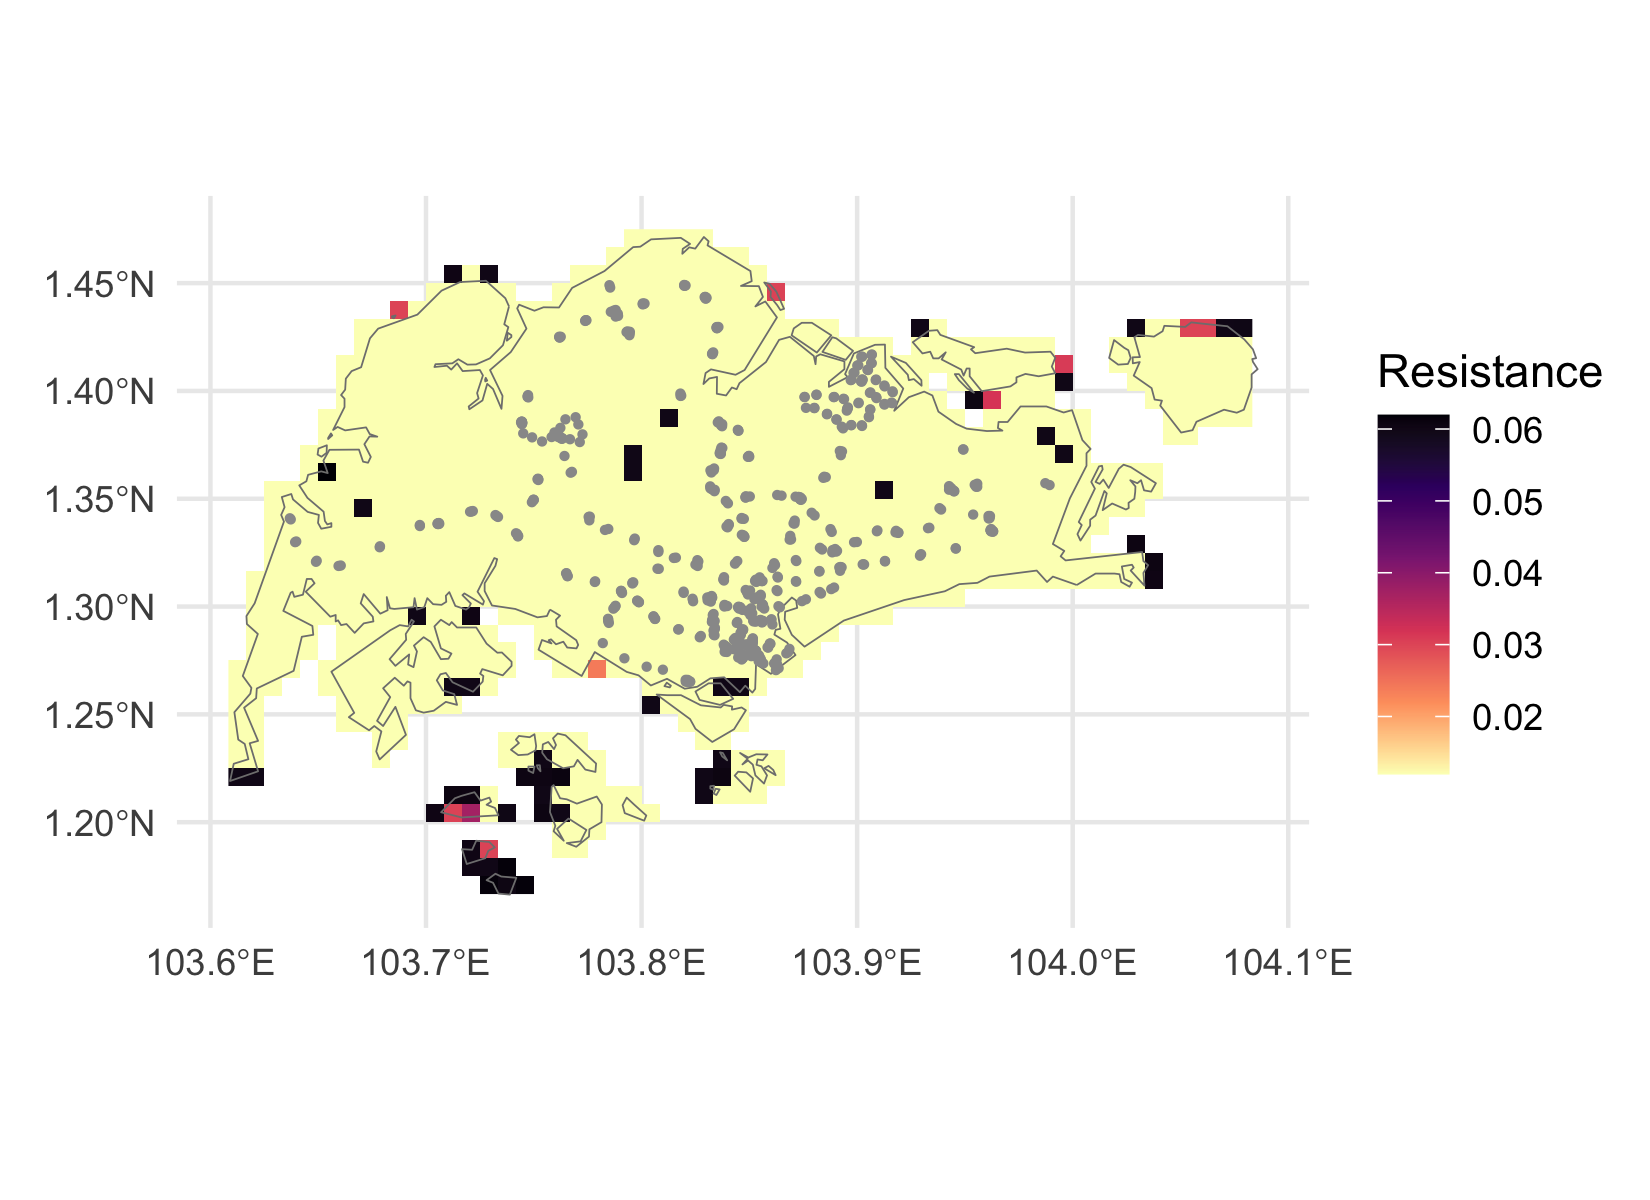
\includegraphics{paper_files/figure-pdf/fig-data-1.png}

}

\caption{\label{fig-data}Friction surface raster of Singapore, showing
Singapore boundary in grey, and station locations as grey points.}

\end{figure}%

\subsection{Calculate and plot the travel
time}\label{calculate-and-plot-the-travel-time}

With all the data collected, the function
\texttt{calculate\_travel\_time()} takes the friction surface
\texttt{friction\_singapore} and the points of interest in
\texttt{stations}, and returns a \texttt{SpatRaster} of walking time in
minutes to each cell from the nearest station:

\begin{Shaded}
\begin{Highlighting}[]
\NormalTok{trave\_time\_singapore }\OtherTok{\textless{}{-}} \FunctionTok{calculate\_travel\_time}\NormalTok{(}
  \AttributeTok{friction\_surface =}\NormalTok{ friction\_singapore,}
  \AttributeTok{points =}\NormalTok{ stations}
\NormalTok{)}

\NormalTok{trave\_time\_singapore}
\end{Highlighting}
\end{Shaded}

\begin{verbatim}
class       : SpatRaster 
dimensions  : 37, 57, 1  (nrow, ncol, nlyr)
resolution  : 0.008333333, 0.008333333  (x, y)
extent      : 103.6083, 104.0833, 1.166667, 1.475  (xmin, xmax, ymin, ymax)
coord. ref. :  
source(s)   : memory
name        : travel_time 
min value   :           0 
max value   :         Inf 
\end{verbatim}

We present the resulting calculated travel times in Figure
Fig~\ref{fig-result} where, as expected, the travel times are lowest
near station exits (per Figure Fig~\ref{fig-data}) and progressively
higher further away. Note that the results in
\texttt{trave\_time\_singapore} include infinite values (\texttt{Inf}
above). In Figure Fig~\ref{fig-data}, the islands to the south and
north-east are shown as filled cells, but unconnected with the mainland.
The raster cells for these islands appear absent in Figure
Fig~\ref{fig-result}. Because they are not connected to any cells with a
station, the calculated travel time is infinite, and so these cells do
not appear in Figure Fig~\ref{fig-result}.

\begin{figure}

\centering{

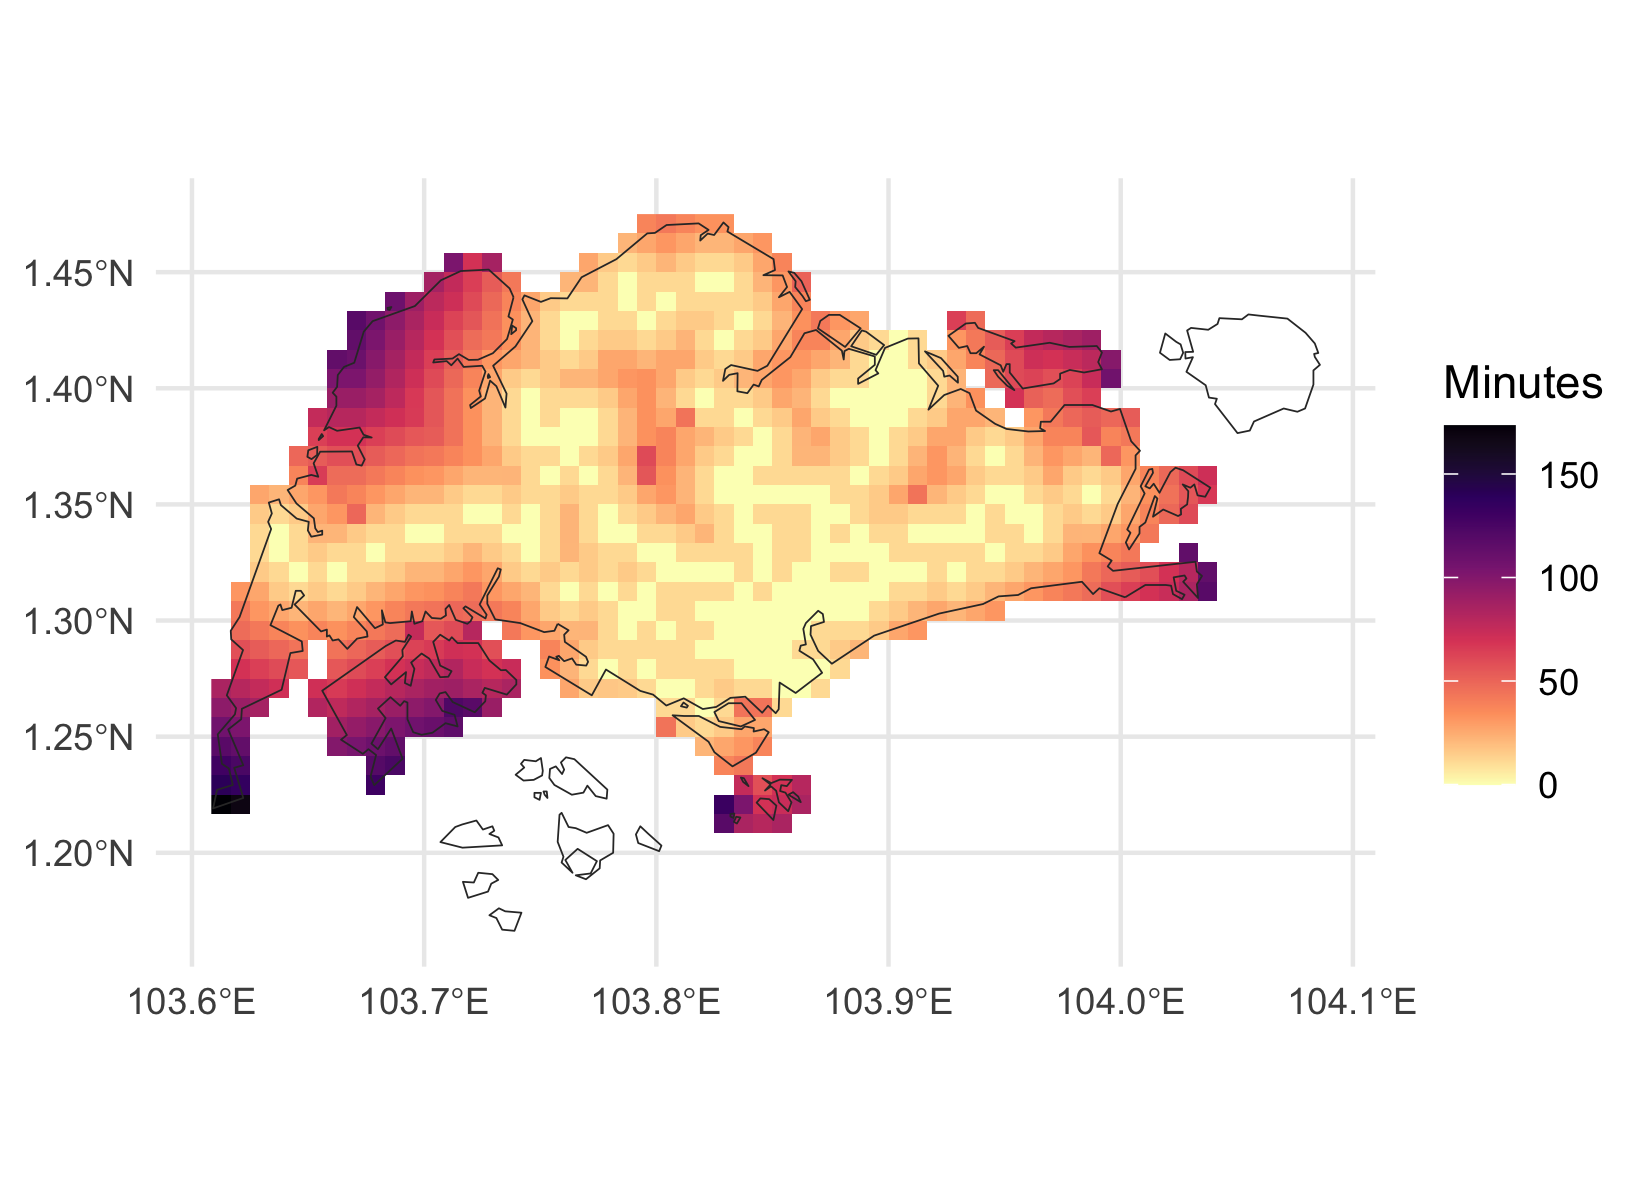
\includegraphics{paper_files/figure-pdf/fig-result-1.png}

}

\caption{\label{fig-result}Map of walking travel time in Singapore, in
minutes from nearest MRT or LRT station.}

\end{figure}%

\section{Opportunities for future
development}\label{opportunities-for-future-development}

The \texttt{traveltime} package is immediately suitable to a range of
applications where travel to custom locations is of interest.
Nonetheless, we see opportunities to build the package utility into the
future through two mechanisms: (1) capability to better distribute a
wider range friction surfaces, and (2) additional methods to handle
large spatial extents.

Firstly, \texttt{traveltime} currently has access to walking and
motorised friction surfaces for 2020, both at 30 arc-second
resolution\footnote{Approximately 0.008333 decimal degrees, or just
  below 1 km\(^2\) at the equator}. Although the user can supply their
own friction surface, we expect most applications will use these
existing surfaces given the extensive work needed in creating new ones
\citep{weiss2018global, weiss2020global}. As landscapes are not dynamic,
it may be useful to incorporate updated versions of these friction
surfaces if and when they are available, though this is likely to occur
first through \texttt{malariaAtlas}. Furthermore, although the
resolution of these data is likely to be suitable for larger landscape
foci, higher resolution data may be helpful for more locally focussed
analyses. For instance, although the example here was chosen for it's
simplicity and low computational demands, a \textasciitilde1
km\textsuperscript{2} cell size is a relatively large area to walk
across, and thus actual waking times may vary significantly within each
cell. We underline however that a user can provide their own higher
resolution friction surface at present if desired.

At the other end of the scale, the calculations can require relatively
large amounts of onboard memory for analyses over large landscapes
(e.g.~analyses over Africa required \textasciitilde{} 72 GB RAM).
Developing methods to handle large landscapes either with less memory or
via cloud resources would be helpful to make such analyses accessible to
those without access to larger computing resources.

\section{Acknowledgements}\label{acknowledgements}

This work was supported, in whole or in part, by the Bill \& Melinda
Gates Foundation {[}INV-021972{]}. The conclusions and opinions
expressed in this work are those of the authors alone and shall not be
attributed to the Foundation. Under the grant conditions of the
Foundation, a Creative Commons Attribution 4.0 License has already been
assigned to the Author Accepted Manuscript version that might arise from
this submission. Please note works submitted as a preprint have not
undergone a peer review process.


% \nolinenumbers
\renewcommand\refname{References}
  \bibliography{paper.bib}


\end{document}
